\chapter{光合作用}\label{ch:g12:photosynthesis}

取一小段金鱼藻倒插于盛水的广口瓶中，置于灯下，
切口处便有气泡成串冒出：是氧气，每隔几秒一个，
灯移近时冒得更快，关灯后便停止。
这种气体是一个过程的可见部分，该过程
养育着地球上每一种动物，也使空气变得可以呼吸，
这已是二十亿年前的事。在\cref{ch:g10:cell-metabolism}中，
这一过程曾用一句话概括：二氧化碳和水在光照下变成糖和氧气。
本章将打开\omterm{def:g12:photosynthesis:chloroplast}{叶绿体}，追踪一个光子的能量
直至化学键中。

\section{叶绿体}

\begin{definition}[叶绿体]\label{def:g12:photosynthesis:chloroplast}
\emph{叶绿体}\index{叶绿体}是\omterm{def:g10:cell-metabolism:autotrophy}{光合作用}的\omterm{def:g10:cells-common-unit:organelle}{细胞器}，
呈透镜形，长约 \qty{5}{\micro m}，外被双层膜，
内有液体，即\emph{基质}，其中
散布着扁平膜囊堆叠而成的\emph{类囊体}\index{类囊体}。
类囊体膜上有色素——\emph{叶绿素} a
和 b（绿色）、橙色的类胡萝卜素——以及
转换光能的\omterm{def:g11:gene-expression:protein}{蛋白质}；基质中则含有合成糖的酶。
一个叶\omterm{def:g10:cells-common-unit:cell}{细胞}中含有数十个叶绿体，一平方毫米的叶片
中约含有五十万个。
\end{definition}

\begin{omfigure}
\begin{tikzpicture}
  \node[anchor=south west, inner sep=0] (img) at (0,0)
    {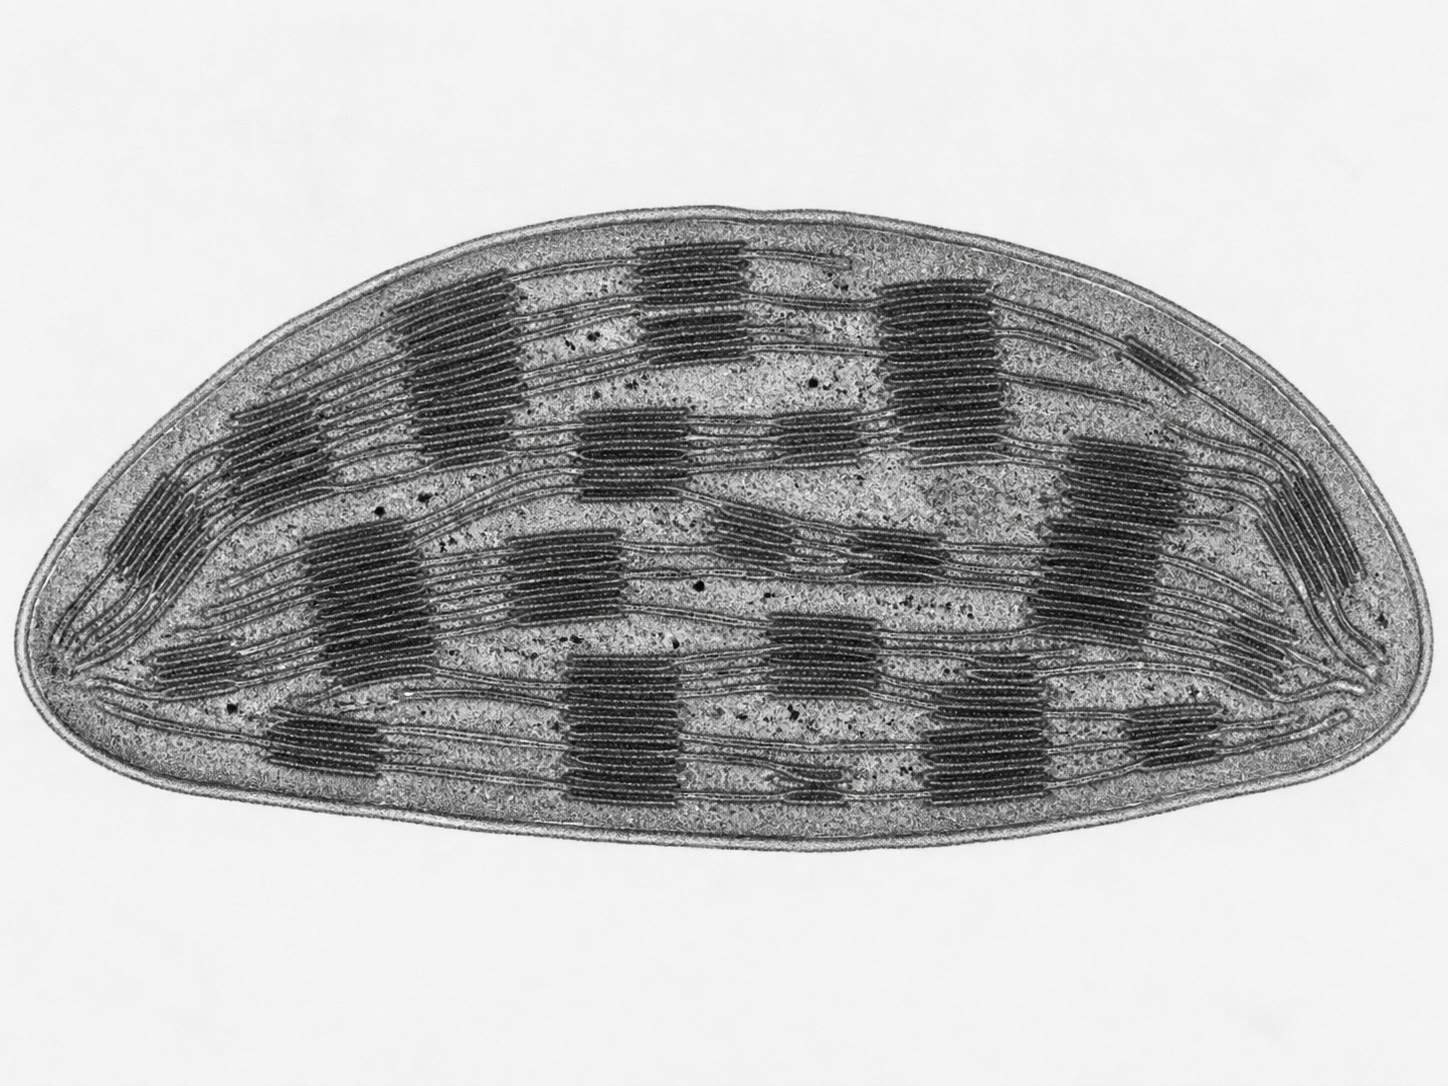
\includegraphics[width=0.5\linewidth]{images/book2/ai/g12-photo-chloroplast-tem.jpg}};
  \begin{scope}[x={(img.south east)}, y={(img.north west)},
      every node/.style={font=\small}]
    \draw[omDef, thick] (0.10,0.50) -- (-0.04,0.80) node[left, align=right] {双层 \\ 包膜};
    \draw[omDef, thick] (0.47,0.72) -- (0.47,1.06) node[above] {堆叠的类囊体（基粒）};
    \draw[omDef, thick] (0.62,0.42) -- (1.04,0.20) node[right] {基质};
    \draw[omDef, thick] (0.80,0.60) -- (1.04,0.75) node[right, align=left] {连接基粒的 \\ 膜};
  \end{scope}
\end{tikzpicture}

{\small 电子显微镜下的\omterm{def:g12:photosynthesis:chloroplast}{叶绿体}：双层包膜，
基质，以及堆叠成基粒的\omterm{def:g12:photosynthesis:chloroplast}{类囊体}膜，色素
所在之处。光在膜上被捕获，糖则在周围的
液体中合成。}
\end{omfigure}

\begin{proposition}[光合作用利用哪些光]\label{prop:g12:photosynthesis:spectrum}
叶绿素强烈吸收蓝光和红光，而对绿光几乎
不吸收——这正是叶片呈绿色的原因。\omterm{def:g10:cell-metabolism:autotrophy}{光合作用}
由色素吸收的波长驱动。以波长为横坐标时，其速率
（即\emph{作用光谱}）随色素的吸收而升降，
在蓝光和红光处出现峰值，在
绿光处出现低谷。
\end{proposition}
\begin{proof}[证据]
恩格尔曼（1882 年）将一条绿藻丝放入一滴水中，
水中有趋氧游动的细菌，并通过显微镜将光谱
沿藻丝投射：细菌聚集在被蓝光与红光照亮的
段落周围，避开绿光——
氧气正是在这些颜色的光照射处释放。
现代测量在不同颜色灯光下的氧气释放量，得到的
曲线与之相同，且与所提取色素的吸收光谱
相吻合。
\end{proof}

\begin{omfigure}
\begin{tikzpicture}
\begin{axis}[
  width=0.88\linewidth, height=5.8cm,
  axis x line=bottom, axis y line=left,
  xmin=400, xmax=700, ymin=0, ymax=110,
  xlabel={波长（nm）}, ylabel={占最大值的\%},
  xlabel style={font=\small, at={(axis description cs:0.5,-0.12)}, anchor=north},
  ylabel style={font=\small},
  tick label style={font=\small}, xtick={400,450,500,550,600,650,700}, ytick={0,50,100},
  legend style={at={(0.5,-0.3)}, anchor=north, legend columns=2, font=\small, draw=none},
]
\addplot[thick, omMeth, smooth] coordinates {(400,70) (430,100) (450,75) (480,35) (500,15) (550,8) (600,15) (640,45) (665,90) (680,70) (700,10)};
\addplot[thick, omThm, dashed, smooth] coordinates {(400,65) (430,85) (450,80) (480,55) (500,35) (550,25) (600,35) (640,60) (665,95) (680,100) (700,20)};
\legend{叶片色素的吸收, 光合作用速率（作用光谱）}
\end{axis}
\end{tikzpicture}

{\small 提取出的叶片色素对光的吸收，以及
叶片\omterm{def:g10:cell-metabolism:autotrophy}{光合作用}的速率，二者均随波长变化。两者
在蓝光和红光处达峰值，在绿光处下降：驱动
\omterm{def:g10:cell-metabolism:autotrophy}{光合作用}的光，正是色素所吸收的光。}
\end{omfigure}

\section{光反应：水的分解与能量的储存}

\begin{proposition}[类囊体中发生了什么]\label{prop:g12:photosynthesis:lightphase}
光照下，\omterm{def:g12:photosynthesis:chloroplast}{类囊体}膜中
同时发生以下三件事：
\begin{itemize}
  \item 水分子被\emph{分解}：其中的氧以
        $\mathrm{O_2}$ 形式释放——\omterm{def:g10:cell-metabolism:autotrophy}{光合作用}所释放的氧来自
        水，而非二氧化碳——其中的氢则
        以电子和质子的形式保留下来；
  \item 被吸收光子的能量用于将这些
        电子装载到一种载体分子\emph{还原型 NADP} 上，
        基质将把它用作氢的来源；
  \item 同一能量驱动 \emph{ATP} 的合成。
\end{itemize}
因此，光反应把光能转化为两种化学产物 ATP
和还原型 NADP，并释放氧气作为副产物。此阶段
不涉及二氧化碳。
\end{proposition}
\begin{proof}[证据]
希尔（1937 年）用光照射悬浮于水中的离体\omterm{def:g12:photosynthesis:chloroplast}{叶绿体}，
加入人工电子受体，但不通入二氧化碳：\omterm{def:g12:photosynthesis:chloroplast}{叶绿体}释放出
氧气，并使受体被还原。可见氧气的释放需要光和水，
水，但不需要 $\mathrm{CO_2}$，且与电子的转移
相偶联。鲁宾与卡门（1941 年）用
含有重同位素 $^{18}$O 的水培养藻类：释放的氧是重的
；若供给重二氧化碳与普通水，则不是。氧
气来自水。
\end{proof}

\begin{omfigure}
\begin{tikzpicture}[font=\small, >=Stealth,
  b/.style={draw, rounded corners, align=center, minimum height=1.0cm}]
  % thylakoid box
  \node[b, fill=omMeth!15, text width=3.6cm, minimum height=3.2cm] (thy) at (0,0) {};
  \node[anchor=north, font=\small\bfseries] at (thy.north) {类囊体膜};
  \node[font=\small, align=center] at (0,-0.1) {叶绿素 \\ 吸收光};
  % stroma box
  \node[b, fill=omDef!10, text width=3.6cm, minimum height=3.2cm] (str) at (6.4,0) {};
  \node[anchor=north, font=\small\bfseries] at (str.north) {基质};
  \node[font=\small, align=center] at (6.4,-0.1) {卡尔文循环：\\ $\mathrm{CO_2}$ 固定 \\ 为糖};
  % inputs/outputs
  \draw[->, thick, omProp] (-3.2,1.0) -- (thy.west |- 0,1.0) node[pos=0, left, omProp] {光};
  \draw[->, thick] (-3.2,-0.6) -- (thy.west |- 0,-0.6) node[pos=0, left] {$\mathrm{H_2O}$};
  \draw[->, thick] (thy.south) -- ++(0,-1.0) node[below] {$\mathrm{O_2}$ 释放};
  \draw[->, thick, omThm] (thy.east |- 0,0.7) -- (str.west |- 0,0.7) node[midway, above] {ATP};
  \draw[->, thick, omThm] (thy.east |- 0,-0.3) -- (str.west |- 0,-0.3) node[midway, above] {还原型 NADP};
  \draw[->, thick, gray] (str.west |- 0,-1.1) -- (thy.east |- 0,-1.1) node[midway, below, font=\scriptsize] {载体返回};
  \draw[->, thick] (9.6,0.6) -- (str.east |- 0,0.6) node[pos=0, right] {$\mathrm{CO_2}$};
  \draw[->, thick] (str.east |- 0,-0.6) -- (9.6,-0.6) node[right] {糖};
\end{tikzpicture}

{\small \omterm{def:g10:cell-metabolism:autotrophy}{光合作用}的两个阶段。在\omterm{def:g12:photosynthesis:chloroplast}{类囊体}膜中，
光分解水、释放氧气，并使两种载体 ATP 和
还原型 NADP 充能。在基质中，这些载体为二氧化碳
固定为糖提供能量。第一阶段需要光；第二阶段
只需要前一阶段的产物。}
\end{omfigure}

\section{碳阶段：糖的合成}

\begin{proposition}[卡尔文循环]\label{prop:g12:photosynthesis:calvin}
在基质中，二氧化碳逐个分子地与
一种已存在的五碳糖结合，由地球上最丰富的
酶催化；六碳产物随即分裂为两个三碳
分子，它们被还原——借助光反应阶段的 ATP 和还原型 NADP——
为三碳糖。其中大部分
被回收，用以再生五碳受体，从而闭合
\emph{卡尔文循环}\index{卡尔文循环}；六个中有一个离开循环
作为植物的净增益。循环三轮，固定三个
$\mathrm{CO_2}$，消耗九个 ATP 和六个还原型 NADP，输出一个三碳糖。
其中两个可合成一个葡萄糖。
\end{proposition}
\begin{proof}[证据]
卡尔文（1950 年代）用放射性
$^{14}$C 标记的二氧化碳供给藻类数秒，随后将它们投入沸腾的酒精中杀死，并
分离其中的分子：五秒后，标记出现在一种
三碳酸中；三十秒后，标记出现在三碳糖和
五碳受体中；数分钟后，标记出现在蔗糖和淀粉中。切断
光照，则受体无法再生，三碳酸
不断积累；切断 $\mathrm{CO_2}$，则受体
不断积累。出现的先后顺序即为循环的顺序。
\end{proof}

\begin{omfigure}
\begin{tikzpicture}[font=\small, >=Stealth]
  \draw[thick, ->] (90:2.2) arc (90:-30:2.2);
  \draw[thick, ->] (-30:2.2) arc (-30:-150:2.2);
  \draw[thick, ->] (-150:2.2) arc (-150:-270:2.2);
  \node[draw, rounded corners, fill=omDef!12, align=center, font=\small] at (90:2.2) {五碳受体 \\ （$\times 3$）};
  \node[draw, rounded corners, fill=omProp!15, align=center, font=\small] at (-30:2.2) {三碳酸 \\ （$\times 6$）};
  \node[draw, rounded corners, fill=omMeth!15, align=center, font=\small] at (-150:2.2) {三碳糖 \\ （$\times 6$）};
  \draw[->, thick] (3.6,2.2) -- (2.4,1.6) node[pos=0, right, align=left] {$3\,\mathrm{CO_2}$ 进入};
  \draw[->, thick, omThm] (2.2,-2.4) -- (1.2,-2.0) node[pos=0, right, omThm, align=left] {6 个 ATP、6 个还原型 NADP\\ 来自光反应阶段};
  \draw[->, thick, omThm] (-3.6,1.0) -- (-2.2,1.4) node[pos=0, left, omThm] {3 个 ATP};
  \draw[->, thick] (-2.4,-2.4) -- (-3.6,-3.2) node[anchor=north, align=center] {1 个三碳糖离开：\\ 半分子葡萄糖};
  \node[font=\scriptsize, align=center] at (0,0) {6 个糖中有 5 个 \\ 用于再生 \\ 3 个受体};
\end{tikzpicture}

{\small \omterm{prop:g12:photosynthesis:calvin}{卡尔文循环}，按三轮计算。三个二氧化碳
分子与三个五碳受体结合；六个三碳产物
被还原为糖，耗用光反应阶段的 ATP 与
还原型 NADP；其中五个再循环为受体，
一个为净增益。}
\end{omfigure}

\begin{example}[葡萄糖的核算]\label{ex:g12:photosynthesis:bookkeeping}
合成一个葡萄糖需要六个二氧化碳分子，故需循环六轮，
共需 18 个 ATP 和 12 个还原型 NADP，均由光反应阶段提供，光反应
分解 12 个水分子，并释放六个氧分子。总反应为：
$6\,\mathrm{CO_2} + 12\,\mathrm{H_2O} \to \mathrm{C_6H_{12}O_6} +
6\,\mathrm{O_2} + 6\,\mathrm{H_2O}$——即
\cref{ch:g10:cell-metabolism}中的总反应式，但此时水分子出现在两侧，
因为释放的氧来自被分解的水，而非来自
二氧化碳。
\end{example}

\begin{omfigure}
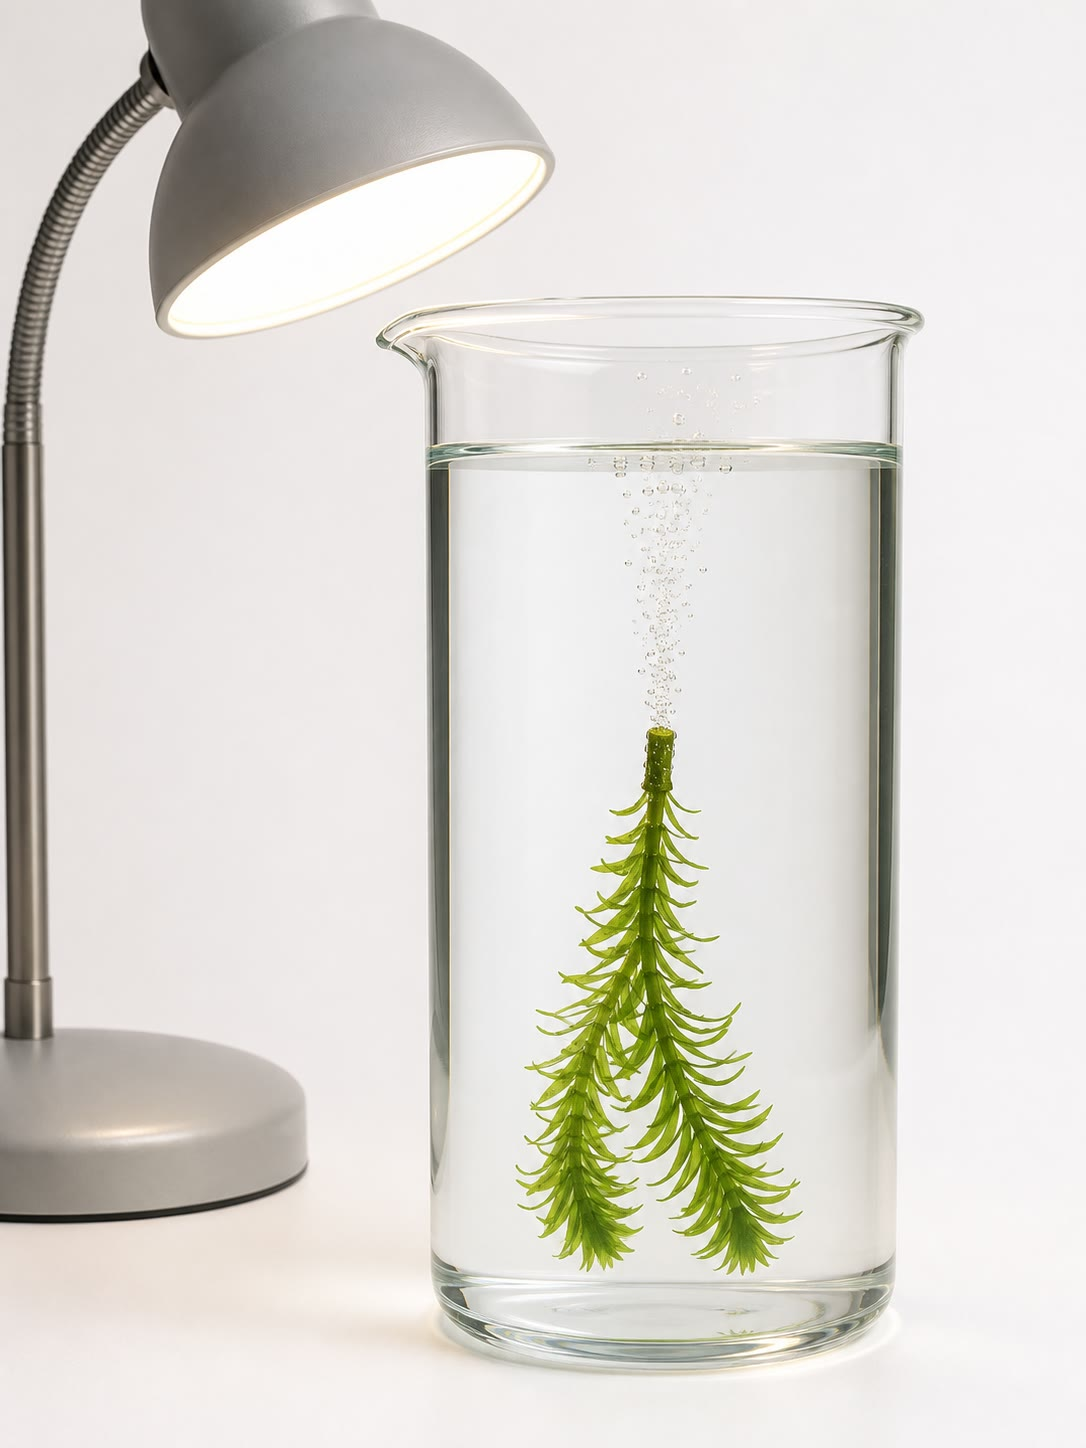
\includegraphics[width=0.34\linewidth]{images/book2/ai/g12-photo-elodea-bubbles.jpg}

{\small 灯下的金鱼藻：从切断的茎中升起的气泡
即光反应阶段释放的氧气。每分钟计数，移动灯具，
改变其颜色，即可测定\omterm{def:g10:cell-metabolism:autotrophy}{光合作用}的速率。}
\end{omfigure}

\section{糖的去向与数量}

\begin{proposition}[产物的去向]\label{prop:g12:photosynthesis:fates}
离开循环的三碳糖在\omterm{def:g12:photosynthesis:chloroplast}{叶绿体}中
被合成为\emph{淀粉}，即叶片的白天储备，或被运出
至\omterm{def:g10:cells-common-unit:cell}{细胞质}，并转化为\emph{蔗糖}，即\omterm{prop:g12:plant-rooted-life:saps}{韧皮部}
所运输的糖（见\cref{ch:g12:plant-rooted-life}）。植物由此
还能制造其他物质：\omterm{def:g10:cells-common-unit:organelle}{细胞壁}所需的纤维素、\omterm{def:g10:chemistry-of-life:families}{脂质}，以及——借助
土壤中的氮和硫——合成\omterm{def:g10:chemistry-of-life:families}{氨基酸}和\omterm{def:g10:universal-dna:nucleotide}{核苷酸}。\omterm{def:g10:cell-metabolism:autotrophy}{光合作用}
不仅是植物能量的来源，也是其全部\omterm{def:g10:chemistry-of-life:mineral-organic}{有机物}
的来源，并通过食物链，成为地球上几乎全部
\omterm{def:g10:chemistry-of-life:mineral-organic}{有机物}的来源。
\end{proposition}
\admitted

\begin{example}[效率：从叶到星球]\label{ex:g12:photosynthesis:efficiency}
满日照每平方米约提供 \qty{1000}{W}，其中
约 45\% 处于色素可利用的波长范围内；叶片
至多将其中约 5\% 在白天转化为糖，而作物在一个
季节内将总日照的 1\% 至 2\% 转为生物量。这一比例虽小，
但总量十分可观：\omterm{def:g10:cell-metabolism:autotrophy}{光合作用}每年固定约
\qty{1e11}{t} 碳——约为大气中碳的七分之一——
并释放出呼吸作用、燃烧和
铁锈所消耗的氧气。
\end{example}

\begin{method}[分析光合作用实验]\label{met:g12:photosynthesis:experiment}
\begin{enumerate}
  \item 确定测量的对象：释放的氧气（光反应阶段），
        吸收的二氧化碳或形成的糖（碳反应阶段），或
        生物量（整体，随时间变化）。
  \item 确定改变的因素：光照（强度、颜色）、二氧化碳、
        温度、水——以及它作用于哪个阶段。
  \item 注意植物同时进行呼吸作用：测得的氧气释放量
        等于\omterm{def:g10:cell-metabolism:autotrophy}{光合作用}产量减去呼吸作用消耗量；在黑暗中，
        只能观察到呼吸作用（见\cref{ch:g10:cell-metabolism}）。
  \item 追踪标记：水中的 $^{18}$O 会出现在氧气中；带 $^{14}$C 标记的
        二氧化碳会依次出现在\omterm{def:g10:chemistry-of-life:families}{糖类}中，
        顺序与循环的先后一致。
\end{enumerate}
\end{method}

\begin{remark}[先光后化]\label{rem:g12:photosynthesis:light}
\omterm{def:g10:cell-metabolism:autotrophy}{光合作用}中唯一需要光的步骤是第一步：
将电子从水转移到载体上，同时释放出
氧气。此后的一切——ATP 的合成、二氧化碳的固定、
糖的合成——都属于化学过程，可在
黑暗中继续进行，只要载体尚有存余；而下一章的呼吸作用
恰好将其逆转。\omterm{def:g12:photosynthesis:chloroplast}{叶绿体}将阳光
转化为化学能的“通货”；\omterm{def:g10:cells-common-unit:cell}{细胞}的其余部分，以及
整个生物圈，则负责消耗它。
\end{remark}

\section{练习}

\begin{exercise}[$\star$]\label{exo:g12:photosynthesis:1}
描述\omterm{def:g12:photosynthesis:chloroplast}{叶绿体}，并说明色素与
\omterm{def:g10:chemistry-of-life:families}{糖类}合成酶分别位于何处。
\end{exercise}

\begin{exercise}[$\star$]\label{exo:g12:photosynthesis:2}
为什么叶片是绿色的？哪些颜色的光最有利于\omterm{def:g10:cell-metabolism:autotrophy}{光合作用}？
\end{exercise}

\begin{exercise}[$\star$]\label{exo:g12:photosynthesis:3}
列出光反应阶段的三种产物，并说明其中哪一种是
副产物。
\end{exercise}

\begin{exercise}[$\star$]\label{exo:g12:photosynthesis:4}
植物释放的氧气来自何处，又
是如何被证明的？
\end{exercise}

\begin{exercise}[$\star$]\label{exo:g12:photosynthesis:5}
合成一分子葡萄糖需要多少个二氧化碳分子、
ATP 分子和还原型 NADP？
\end{exercise}

\begin{exercise}[$\star\star$]\label{exo:g12:photosynthesis:6}
由光谱图读出吸收率与光合速率，
分别在 \qty{550}{nm} 和 \qty{665}{nm} 处的数值。温室为节约能源改用
绿色灯照明，请对此作出评论。
\end{exercise}

\begin{exercise}[$\star\star$]\label{exo:g12:photosynthesis:7}
逐步解释恩格尔曼的实验：细菌检测到的是什么，
它们为何聚集在那些位置，以及该实验
说明了什么。
\end{exercise}

\begin{exercise}[$\star\star$]\label{exo:g12:photosynthesis:8}
将离体\omterm{def:g12:photosynthesis:chloroplast}{叶绿体}置于水中，在光照下，加入人工电子受体
且不提供 $\mathrm{CO_2}$，仍能释放氧气。这说明
氧气释放与碳固定之间
存在怎样的关系？
\end{exercise}

\begin{exercise}[$\star\star$]\label{exo:g12:photosynthesis:9}
在卡尔文的实验中，关闭光照而 $\mathrm{CO_2}$
仍继续通入：三碳酸积累，五碳受体
消失。试解释这两种现象。
\end{exercise}

\begin{exercise}[$\star\star$]\label{exo:g12:photosynthesis:10}
一株水草在距灯 \qty{20}{cm} 处，每分钟释放 30 个气泡；
在距灯 \qty{40}{cm} 处则释放 8 个。试解释原因，并预测
其在黑暗中的气泡数。
\end{exercise}

\begin{exercise}[$\star\star$]\label{exo:g12:photosynthesis:11}
一片叶子每平方米每小时固定 \qty{8}{g} 的 $\mathrm{CO_2}$。
这相当于多少质量的葡萄糖，又释放出
多少质量的氧气？（摩尔质量：$\mathrm{CO_2}$ 44，葡萄糖 180，$\mathrm{O_2}$ 32，
单位为 \unit{g/mol}。）
\end{exercise}

\begin{exercise}[$\star\star\star$]\label{exo:g12:photosynthesis:12}
解释碳反应阶段为何常被称为“暗反应”，并说明
这一名称为何具有误导性，可借助将植物置于黑暗中一小时后
所发生的变化来说明。
\end{exercise}

\begin{exercise}[$\star\star\star$]\label{exo:g12:photosynthesis:13}
给植物提供标记 $^{18}$O 的水与标记
$^{14}$C 的二氧化碳。请说明两种标记在
一分钟后、一小时后和一天后分别出现在何处。
\end{exercise}

\begin{exercise}[$\star\star\star$]\label{exo:g12:photosynthesis:14}
满日照提供 \qty{1000}{W/m^2}，一片叶子以糖的形式储存其中的
\qty{20}{W/m^2}。计算其效率；然后
列出其余能量去向的三个地方。
\end{exercise}

\begin{exercise}[$\star\star\star$]\label{exo:g12:photosynthesis:15}
大气中的氧气（21\%）完全来源于
\omterm{def:g10:cell-metabolism:autotrophy}{光合作用}。试解释为何没有\omterm{def:g10:cell-metabolism:autotrophy}{光合作用}的地球会在
数千年内失去其中的氧气，并说明这对地球最初的
二十亿年意味着什么。
\end{exercise}

\section{问题：一平方米叶片}

\begin{problem}[{周末问题——追踪阳光能量转化为糖的过程：
计数光子，核算载体，平衡氧与碳，
并计算叶片的效率}]
\label{pb:g12:photosynthesis:1}
一平方米处于满日照下的叶片接收 \qty{1000}{W}，其中
\qty{450}{W} 位于色素所吸收的波长范围内；该叶片每小时固定
\qty{8}{g} 的 $\mathrm{CO_2}$。葡萄糖每摩尔储存
\qty{2870}{kJ} 的能量。摩尔质量：$\mathrm{CO_2}$ 为 44，$\mathrm{O_2}$ 为 32，
$\mathrm{H_2O}$ 为 18，葡萄糖为 \qty{180}{g/mol}。

\medskip
\noindent\textbf{第一部分——碳与氧。}
\begin{enumerate}
  \item 叶片每小时固定多少摩尔的 $\mathrm{CO_2}$？
  \item 由此可生成多少摩尔、多少克葡萄糖？
  \item 释放出多少摩尔的 $\mathrm{O_2}$，其体积为多少
        （每摩尔 \qty{24}{L}）？
  \item 为释放这些氧气，需分解多少个水分子？
        这一数量与一平方米叶片在一小时内蒸腾的
        \qty{600}{mL} 水相比如何？
  \item 所释放的 $\mathrm{O_2}$ 中，每个氧原子
        来自何处，你如何得知？
\end{enumerate}

\medskip
\noindent\textbf{第二部分——载体。}
\begin{enumerate}[resume]
  \item 每小时需要进行多少轮\omterm{prop:g12:photosynthesis:calvin}{卡尔文循环}？
  \item 光反应时期每小时可提供多少 ATP，以及多少
        还原型 NADP？
  \item 每个还原型 NADP 携带的两个电子取自水。每小时
        需分解多少个水分子才能提供这些电子？
        与第 4 题相比。
  \item 若叶片的光反应时期停止（比如\omterm{def:g12:photosynthesis:chloroplast}{叶绿体}被毒害而不能分解水），
        则 ATP、还原型 NADP、氧气和\omterm{def:g10:chemistry-of-life:families}{糖类}中，哪些会停止生成，
        且以何种顺序停止？
  \item 若改为去除 $\mathrm{CO_2}$，
        光反应时期会在数秒内发生什么变化？为何如此？
\end{enumerate}

\medskip
\noindent\textbf{第三部分——能量。}
\begin{enumerate}[resume]
  \item 计算每小时所生成葡萄糖中储存的能量，
        以千焦表示，再以瓦特表示为功率。
  \item 计算该叶片相对于满日照的效率，
        以及相对于所吸收波长的效率。
  \item 一个红光光子（\qty{680}{nm}）约携带
        \qty{176}{kJ}（每摩尔光子）。固定一个 $\mathrm{CO_2}$
        约需 8 个光子。计算所用光子的能量
        （每摩尔 $\mathrm{CO_2}$），并与每摩尔 $\mathrm{CO_2}$
        固定后所储存的能量（$2870/6$）相比较。
  \item 被吸收光子的能量中，有多大比例最终进入
        葡萄糖？其余部分去向何处？
  \item 该叶片每小时还将进行呼吸作用，消耗 \qty{0.5}{g} 葡萄糖。其净增益
        为多少？你将如何测量它？
\end{enumerate}

\medskip
\noindent\textbf{第四部分——从叶片到地球。}
植物每年固定约 \qty{1e11}{t} 的碳；大气中
约有 \qty{8.5e11}{t} 的碳以 $\mathrm{CO_2}$ 形式存在；海洋中的藻类
固定的碳量与陆地植物大致相当。
\begin{enumerate}[resume]
  \item 若没有任何过程使碳返回空气中，\omterm{def:g10:cell-metabolism:autotrophy}{光合作用}需要
        多少年才能将大气中的 $\mathrm{CO_2}$ 耗尽？
  \item 说出使碳返回大气的过程，并解释为何
        直到不久以前，大气中的 $\mathrm{CO_2}$ 含量
        大致保持稳定。
  \item 计算固定 \qty{1e11}{t} 碳时每年释放的氧气质量
        （每个碳对应一个 $\mathrm{O_2}$）。
  \item 大气中约含 \qty{1.2e15}{t} 氧气。这相当于
        多少年的\omterm{def:g10:cell-metabolism:autotrophy}{光合作用}产量？为何此答案不等于
        氧气的年龄？
  \item 归纳结论：该平方米叶片的效率，
        它所释放氧气的来源，以及每年
        通过叶片的大气碳所占的比例。
\end{enumerate}
\end{problem}
